% !TEX root = ../master-thesis.tex

\begin{figure}
    \centering
    % 
    \addletter{140}{a} 
    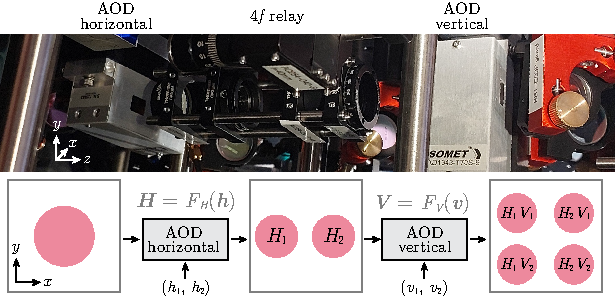
\includegraphics{fig-ai/crossed-aod.pdf}
    \hfill
    \addletter{140}{b} 
    \includegraphics{fig-py/crosstalk-camera.pdf}
    % 
    \newline
    \phantom{42}
    \newline
    % 
    \addletter{115}{c}
    \raisebox{1cm}{\includegraphics{fig-py/crosstalk-camera-img.pdf}}
    \phantom{42}
    \addletter{115}{d}
    \includegraphics{fig-py/crosstalk-camera-amp.pdf}  
    \phantom{42}
    \addletter{115}{e}
    \includegraphics{fig-py/crosstalk-camera-res.pdf}
    % 
    \caption{
        \textbf{Tweezer array control using orthogonal AODs.}
        (a) Experimental setup: two orthogonal AODs generate a 2D tweezer array. The applied harmonic amplitudes $h_i$, $v_j$ define the output intensities $H_i = F_H(h)$ and $V_j = F_V(v)$ in horizontal and vertical directions, respectively. 
        (b) Crosstalk matrix $F'$ reconstructed via linear regression from camera images, showing how modulation of one harmonic affects others. 
        (c) Example of measured intensity distribution at uniform input amplitudes ($h_i = v_j = 0.9$), illustrating imbalance in the resulting pattern. 
        (d) The total intensity $\Lambda = \sum_{ij} H_i V_j$ scales linearly with the mean input amplitude. 
        (e) Residuals of the linear model (fitted in the range $[0.85, 0.95]$) are normally distributed. 
        All data were obtained in this work using direct camera-based measurements.
    }
    \label{fig:control}
\end{figure}


Optical tweezer arrays provide a flexible platform for preparing ultracold atomic systems with site-resolved control. By trapping individual atoms in focused laser beams, it becomes possible to initialize many-body states with controlled geometry, low entropy, and tunable local parameters.

In our setup, a two-dimensional array of tweezers is created using two orthogonal acousto-optic deflectors (AODs). Each AOD diffracts multiple beams along one axis, and their intersection forms the full array. The resulting intensity at site $(i,j)$ factorizes as $P_{ij} = H_i V_j$, where $H_i$ and $V_j$ are set by the drive amplitudes applied to each AOD. This structure simplifies calibration and allows fast control of the entire array using a small number of parameters.

Compared to holographic or lattice-based approaches, the AOD system offers rapid reconfigurability and independent control of individual traps. This enables preparation of custom spin and density patterns, as well as dynamic manipulation during the experimental sequence. Such capabilities are useful, for example, for initializing specific configurations, removing defects, or performing spatially selective operations before loading atoms into an optical lattice for further evolution.

\textbf{AOD operation.} Each AOD consists of a crystal driven by a piezoelectric transducer. An incoming laser beam $(\vc{k}_{\mathrm{in}}, \omega_{\mathrm{in}})$ interacts with the induced acoustic wave $(\vc{q}, \Omega)$ via Bragg diffraction, producing an outgoing beam $(\vc{k}_{\mathrm{out}}, \omega_{\mathrm{out}})$:
\begin{equation*}
    \vc{k}_{\mathrm{out}} = \vc{k}_{\mathrm{in}} + \vc{q}, \qquad \omega_{\mathrm{out}} = \omega_{\mathrm{in}} + \Omega.
\end{equation*}
The frequency $\Omega$ determines the deflection angle $\theta$ through the Bragg condition, while the amplitude of the RF signal controls the diffracted optical power. Each RF tone can be described by a triple $(\Omega_j, a_j, \varphi_j)$, corresponding to its frequency, amplitude, and phase. Applying a set of such tones to an AOD results in a superposition of multiple diffracted beams, with the amplitude $a_j$ determining the power in each beam and the phase $\varphi_j$ influencing their relative coherence.


\textbf{Factorized intensity distribution.} 
To create 2D arrays, we combine two AODs oriented along orthogonal axes (fig.~\ref{fig:control}a), as described in~\cite{culemann_construction_2024}.
Each axis is driven by a set of RF tones. In the paraxial approximation, the resulting 2D intensity pattern can be written as a rank-1 product of two vectors:
\begin{equation*}
    P_{ij} = H_i V_j,
\end{equation*}
where $H_i$ and $V_j$ correspond to the powers of individual beams generated by the horizontal and vertical AOD, respectively. The factorization of the output power can be verified via:
\begin{equation}
\label{eq:factorisability}
    P \overset{\mathrm{SVD}}{=} \textstyle \sum_r \Lambda_r \vc{H}_r \vc{V}_r\T,
    \hspace{10 mm} 
    \text{factorisability} = \Lambda_0 / \sum_r \Lambda_r 
\end{equation}
which provides a natural measure of factorization. For arrays ranging from $2\times2$ to $10\times10$, the factorisability measure $\Lambda_0 / \sum_r \Lambda_r$ is consistently above $0.99$. For the $4\times4$ array used in most of our experiments, we obtain a typical value of $0.997(1)$.

\textbf{Tweezer array control.} The tweezer output beam powers are nonlinear functions of the input amplitudes $\vc{a}$:
\begin{equation}
    \label{eq:taylerexp}
    P_j = F_j(\vc{a}) = \cancel{F_j(\vc{0})} + F'_{ji} a_i + \tfrac{1}{2} F''_{j i_1 i_2} a_{i_1} a_{i_2} + \ldots
\end{equation}
The goal is to control\footnote{
    For amplitudes in the range $a_i \in [0.7, 1.0]$, we find that a linear or quadratic approximation suffices. In practice, we reconstruct the Jacobian matrix $F'_{ji}$ using camera-based calibration, as discussed in Sec.~\ref{subsec:control}.
} the full matrix $P_{ij}$ using only two sets of parameters: horizontal amplitudes $\vc{h}$ and vertical amplitudes $\vc{v}$. 

It will later be necessary to reconstruct $(H_i, V_j)$ from measured intensity distribution $P_{ij}$, so it is convenient to choose a factorized model $P_{ij} = \Lambda H_i V_j$, with the normalization:
\begin{equation*}
    \sum_i H_i = \sum_j V_j = 1, \hspace{5 mm} \sum_{ij} P_{ij} = \Lambda.
\end{equation*}
This allows for an explicit decomposition:
\begin{equation}
    \textstyle
    \frac{1}{\Lambda} \sum_j P_{ij} = H_i \sum_j V_j = H_i,
    \hspace{5 mm} 
    \frac{1}{\Lambda} \sum_i P_{ij} = V_j \sum_i H_i = V_j,
    \hspace{5 mm} 
    \sum_{ij} P_{ij} = \Lambda,
    \label{uv-decomposition}
\end{equation}
which is fully equivalent to a rank-1 SVD of $P_{ij}$.

It is worth noting that, as shown in Fig.~\ref{fig:control}d, the total scale parameter $\Lambda$ defined in this way is proportional to the total input amplitude, $\sub{a}{sum} = \sum_j h_j + \sum_j v_j$. This effectively decouples local balancing from global power constraints, simplifying the control problem.

% \grey{This allows us to adjust the global scale $\Lambda$ (via a shared AOM or pre-AOD attenuation) and balance individual amplitudes using only two $n$-dimensional vectors.}
